\documentclass{article}

% if you need to pass options to natbib, use, e.g.:
% \PassOptionsToPackage{numbers, compress}{natbib}
% before loading nips_2017
%
% to avoid loading the natbib package, add option nonatbib:
% \usepackage[nonatbib]{nips_2017}
\usepackage{graphicx}
\usepackage{nips_2017}

% to compile a camera-ready version, add the [final] option, e.g.:
% \usepackage[final]{nips_2017}

\usepackage[utf8]{inputenc} % allow utf-8 input
\usepackage[T1]{fontenc}    % use 8-bit T1 fonts
\usepackage{hyperref}       % hyperlinks
\usepackage{url}            % simple URL typesetting
\usepackage{booktabs}       % professional-quality tables
\usepackage{amsfonts}       % blackboard math symbols
\usepackage{nicefrac}       % compact symbols for 1/2, etc.
\usepackage{microtype}      % microtypography

\title{Neural Networks and Redundancy in Network Layers}

% The \author macro works with any number of authors. There are two
% commands used to separate the names and addresses of multiple
% authors: \And and \AND.
%
% Using \And between authors leaves it to LaTeX to determine where to
% break the lines. Using \AND forces a line break at that point. So,
% if LaTeX puts 3 of 4 authors names on the first line, and the last
% on the second line, try using \AND instead of \And before the third
% author name.

\author{
  Jeremy K. Goens\thanks{ } \\
  Department of Computer Science\\
  South Dakota School Of Mines and Technology\\
  501 E St Joseph St, Rapid City, SD 57701\\
  \texttt{jeremy.goens@mines.sdsmt.edu} \\
  %% examples of more authors
  %% \And
  %% Coauthor \\
  %% Affiliation \\
  %% Address \\
  %% \texttt{email} \\
  %% \AND
  %% Coauthor \\
  %% Affiliation \\
  %% Address \\
  %% \texttt{email} \\
  %% \And
  %% Coauthor \\
  %% Affiliation \\
  %% Address \\
  %% \texttt{email} \\
  %% \And
  %% Coauthor \\
  %% Affiliation \\
  %% Address \\
  %% \texttt{email} \\
}

\begin{document}
% \nipsfinalcopy is no longer used

\maketitle

\begin{abstract}
  This documents is a look into the redundancy of extra neural network layers. This will 
  be an overview of the benefits or the faults of having an extensive amount of layers, first 
  layer Neural Networks without any dropout in the neural network.
\end{abstract}

\section{Deep Learning}

Deep Learning
The study of deep learning is based on the idea of the human brain. It starts off with the idea of making a computer think like a human. This has been the ideal for many years for society, and there have been many different approaches to creating a human-like machine.

To complete this ideal, the idea of the perceptron was created.  The perceptron is an electronic “node” that takes in multiple inputs, each line consisting of a different value from the input line, and a weighted value, that the input will be multiplied. This will create a number that would be between zero and one. This may be used for identification of items, such as handwriting, labels, stock market trends, and, given a large enough network, the ability to mimic certain human like behaviors.
The perceptron helped bring forward the Artificial Intelligence idea of having human like robots forward, however, there was a problem with how many perceptron a computer could contain. This has been a huge wall that the community has not completely overcome, however, over the years, there have been several breakthroughs. A major one being the development of Neural Networks.

\section{Neural Networks}
The development of the Neural Network helped push the envelope of what was possible in the world of Artificial Intelligence. This was completed by taking advantage of the perceptrons that were created by linking them together and treating them like a set of neurons. This helped push this forward for learning when it came to Artificial Intelligence as not only were perceptrons able to identify a single item anymore, but a several layers of them could break up a set of information, be it an image or a multiple data pieces, so that each perceptron could be used to identify smaller sections of an item, increasing the likelihood of identification, or trends within a given market.

 This development lead to several perceptrons that could be used for better identification, such as when attempting to identify numbers. Instead of a single perceptron looking at the image, broken up into different inputs, instead you could have several perceptrons that would break up the same image and attempt to decide if a number is a 4 or a 9, and pull the inputs back in from both perceptrons which would increase the likely hood that you would correctly identify an image as the correct number.
But with Neural Network development, there was a thought that why not layer these networks, passing the inputs from the previous layer into the new one to attempt to increase the correct guess. But before you could attempt a Multi-Layer Neural Network, the network that you were given would need to be trained first. Training a Neural Network, while not difficult, does take an intense amount of information, and an even larger set of data to work through.


\begin{figure}[h]
  \centering
  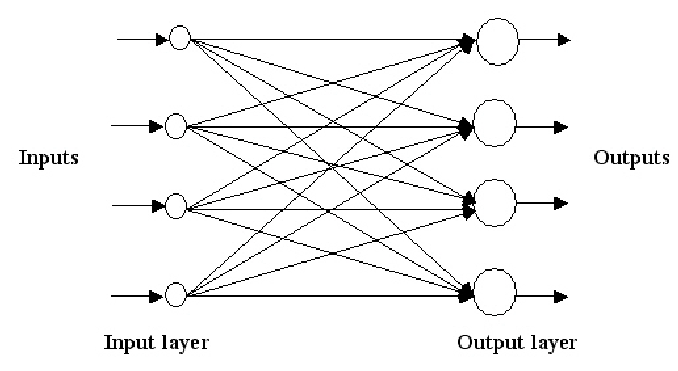
\includegraphics[width=\textwidth]{pics/single_layer.png}
  \caption{Single Layer Neural Network}
\end{figure}



\section{Training a Neural Network}
To train a Neural Network, a large dataset is required. When Neural Networks were new, this meant there were many hours spend collating and combining given information to learn to train a Neural Network. To do this, you take part of a given sample set, and run it through the Neural Network, and when the output is given, if it is correct, you do nothing, but if the output is wrong, you run calculations in reverse to help even out the networks weighting system for each input. This is done by calculating the error that comes from each node in the network, and then adjusting it, given a certain training weight or percent, and adjusting the weight number by the amount of error multiplied by the percentage that is taken.

Given that large datasets are required, this lead to many hours of attempting to even out a network to approach that perfect identification, even given a piece of data that was not included in the training dataset. But with the error still being large, even given expansive inputs for a Neural Network, the attempt at making a Multi-Layer Neural Network was the next approach that was taken to attempt to even out this error that single layers still gave.

\section{Multi-Layer Neural Networks}
Multi-Layer Neural Networks were a very good reinvigoration for the fields of Deep Learning and Neural Networks. What a Multi-Layer Neural Networks consists of are several single layers, some completely connected to the next layer, some that only connect to a handful of the nodes in the next layers that could be used to even easier correctly identify items given enough time and training.

The difficult part of using a neural network is not the direct training, but also, how you will use the given information for each of the layers. Unlike a single layer Neural Network, a Multi-Layer Neural Networks does not take in new information for each layer, but instead after the first layer of nodes process the image, the output is then passed forward into the new layer of nodes which then process it forward. This layer effect can be used for between two to fifteen layers, but typically they do not cover more than that.

The largest restriction on how many layers a given project could use was not restricted by the person working on the development of the network, but again, we ran into a hardware issue. Given that at the time of its development, multi-core processors were unheard of this slowed development for several years. However, with the development of multi-core processors and access to GPU processors that could be used for processing, the speed boost to these networks were unbelievable and still being tested with current technology.

The development of the Multi-Layer Neural Networks helped again push the envelope when it came to identifying a given image. However, this also meant that a new way of training had to be developed, as adjusting the weights on the final layer of the neural Network would only adjust the entire system so much.  

\begin{figure}[h]
  \centering
  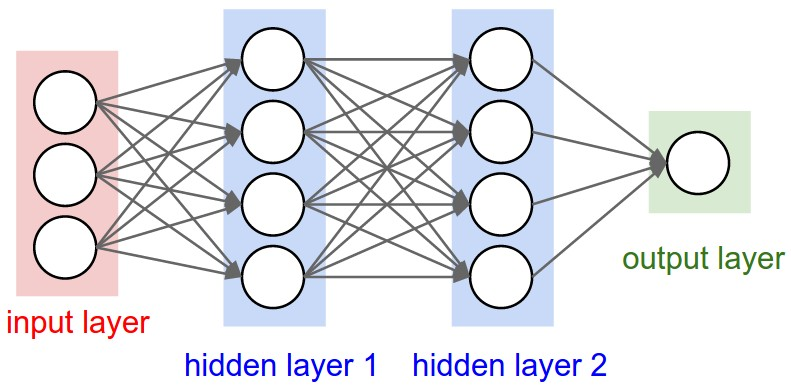
\includegraphics[width=\textwidth]{pics/multi_layer.jpg}
  \caption{Multi-Layer Neural Network}
\end{figure}

\section{Training Multi-Layer Neural Networks}
Since Multi-Layer Neural Networks require several layered Neural Networks, one of the more efficient ways of enhancing the system was to add adjustment to the previous layers. This seemingly worked out very easy in the end. The process still involved adjusting the final Neural Network weights, however, once that is completed, this new error is passed back by each node to the previous layer, and given different weights adjust the next previous layer’s weights. This is repeated for each successive layer until the first layer is reached. From here the Multi-Layer Neural Networks can process new training data, and again attempts a correct identification.

Single Layer vs Multi-layer Neural Networks
The benefits of a Multi-Layer Neural Networks make it seem like an obvious choice when attempting to train a Neural Network, however, there are some benefits that a Single Layer may give you.

\subsection{Training}

Since a Single Layer Neural Network is much faster, completing the training is very simple and helps with completing the trainging very quickly if that is needed. However, this also leads to a greater erro chance when it comes to correctly identifying a given image. The benefits of having quicker training is a system that is up and running much faster.

The Multi-Layer Neural Network on the other hand may be more accurate, but the traiing required and the back propogation for correctly identifying which node is causing error could take may more iteration. However, as the graps below show, the error can be greatly reduced as well.

\begin{figure}[h]
  \centering
  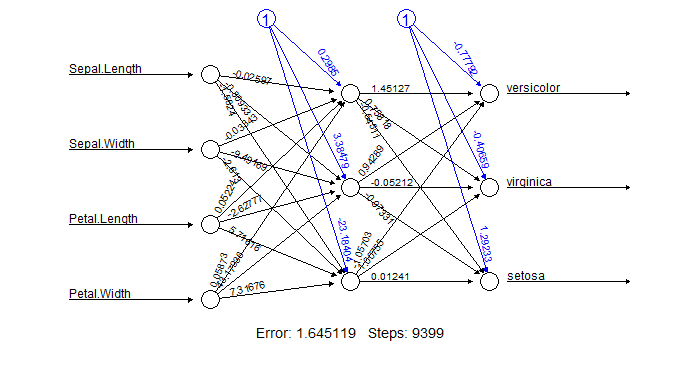
\includegraphics[width=\textwidth]{pics/training.png}
  \caption{Neural Network Training}
\end{figure}

\subsection{Large Datasets}

Having to process large sets of data with a Neural Network can lead to a huge amount of downtime. For a Single Layer Neural Network, this is usually not the problem, as the use of his would indicate a huge amount of error allowed. 

Meanwhile, Multi-layer Neural Networks would take even longer, but because they have such a large dataset, their ability to correctly identify a given image would greatly increase their ability to perform on the system over all. 

\begin{figure}[h]
  \centering
  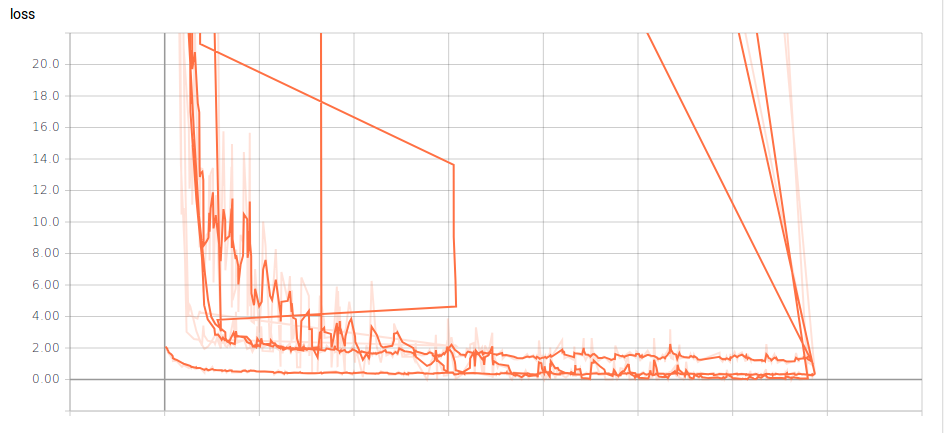
\includegraphics[width=\textwidth]{pics/3layererror.png}
  \caption{3 Layer Error Percent}
\end{figure}

\begin{figure}[h]
  \centering
  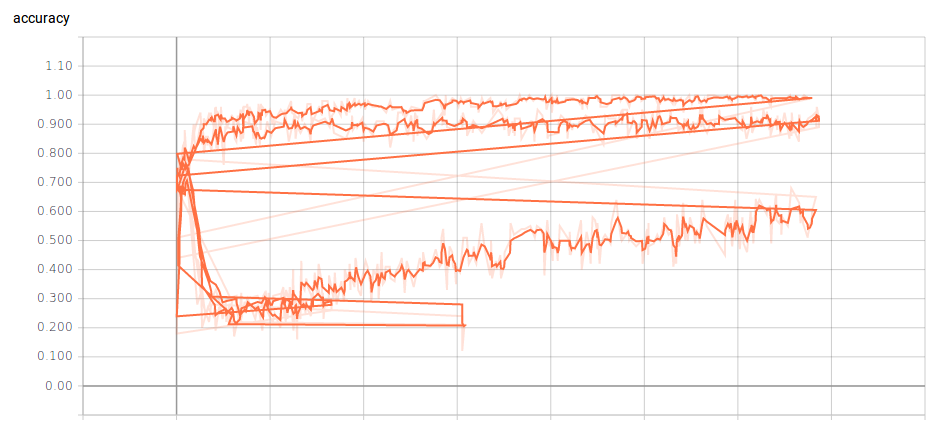
\includegraphics[width=\textwidth]{pics/3layercorrect.png}
  \caption{3 Layer Correct Identification}
\end{figure}

\subsection{Large Training Iteration}
An easy win is pointed out in this area for the Multi-layer Neural Networks as it does take longer, but again, this would be needed to correctly identify a image much more accurately. This is because the Single Layer Network would not be able to correctly train even given a large enough data set.

\section{Redundancy}
Now while Multi-layer Neural Networks have a huge benefits over smaller Single Layer Network, they do suffer from one major issue. Redundancy is a huge problem when it comes to making Multi-layer Neural Networks as to many layers is just as bad as to few. During testing, there were several different multilayer networks ran, once consisting of 15 layers, one consisting of 5 layers, one of 3 layers, and one being a single layer Neural Network. What was shown is more layers than the 5 actually reduced the accuracy with which a item can be identified and also creates problems in correctly identifying the training data set around 135,000 iteration of training.


\section{Testing and Conclusion}
The Single Layer Neural Network worked well when running on its own, but the performance never made it higher than 80\% efficiency when identifying anything outside of the training set.

The 5 Multi-layer Neural Network on the other hand seemed to be able to correclty identify the training dataset at the 134,000 training iteration with 100\% accuracy and the actual tested dataset with 98.74\% accurracy. This was tested against the MNIST handwriting data set to make iteration of training easier.

The 15 Multi-layer Neural Network when tested worked well when training iteration we arond 10,000. However, after an additional 100,000 training  iterations, the percentage of correctly identified images would drop 1-4\% on different run. While this may not seem like much of a drop, the 5 Multi-layer Neural Network never dropped below 96\% identification, even when run with only 100 training iteration.

This may go to represent that while a Multi-layer Neural Network is better than a Single Layer Neural Network, to much work in a Multi-layer Neural Network may be just as harmful to the overall performance of a system as to little.


%\subsubsection*{Acknowledgments}

\section*{References}

\small

[1] David A. Medler \ \& Michael R. W. Dawson\ Using Redundancy to 
Improve the Performance of Artificial Neural Networks*

[2] Micheal Cogswell\ (2016) Thesis submitted to the Faculty of
Virginia Polytechnic Institute and State University {\it  Understanding 
Representations and Reducing their Redundancy in Deep Networks}  

%[3] Hasselmo, M.E., Schnell, E.\ \& Barkai, E.\ (1995) Dynamics of
%learning and recall at excitatory recurrent synapses and cholinergic
%modulation in rat hippocampal region CA3. {\it Journal of
%  Neuroscience} {\bf 15}(7):5249-5262.

\end{document}
